\documentclass[11pt,a4paper,oneside]{book}
\newcommand{\NumeroRelazione}{7}

\newcommand{\TitoloRelazione}{Misure con vector Network Analysers di dispositivi lineari a 2 e 4 porte e di amplificatori}
\usepackage[utf8]{inputenc}       
\usepackage[T1]{fontenc}          
\usepackage[italian]{babel}       
\usepackage{graphicx}             
\usepackage{float}
\usepackage{amsmath}
\usepackage{amsfonts} 
\usepackage{amssymb}  
\usepackage{steinmetz}
\usepackage{pgfplots}
\usepackage{tikz}
\usepackage{enumitem} 
\usepackage{subcaption}
\usepackage{caption}
\usepackage{comment}
\usepackage[normalem]{ulem}
\usepackage[americaninductors, siunitx]{circuitikz}

\usetikzlibrary{arrows.meta, patterns, shapes.geometric, calc, positioning, shapes, arrows}
\pgfplotsset{compat=1.18}

% --- GEOMETRY (Margini e distanze) ---
\usepackage[
    a4paper,
    top=3.5cm,      
    bottom=3cm,    
    left=3cm,      
    right=3cm,     
    headheight=40pt, % Spazio per l'immagine
    headsep=25pt     % Distanza tra immagine e testo/titoli
]{geometry}

% --- FANCYHDR (Intestazioni) ---
\usepackage{fancyhdr} 
\pagestyle{fancy}
\fancyhf{} 
\fancyhead[L]{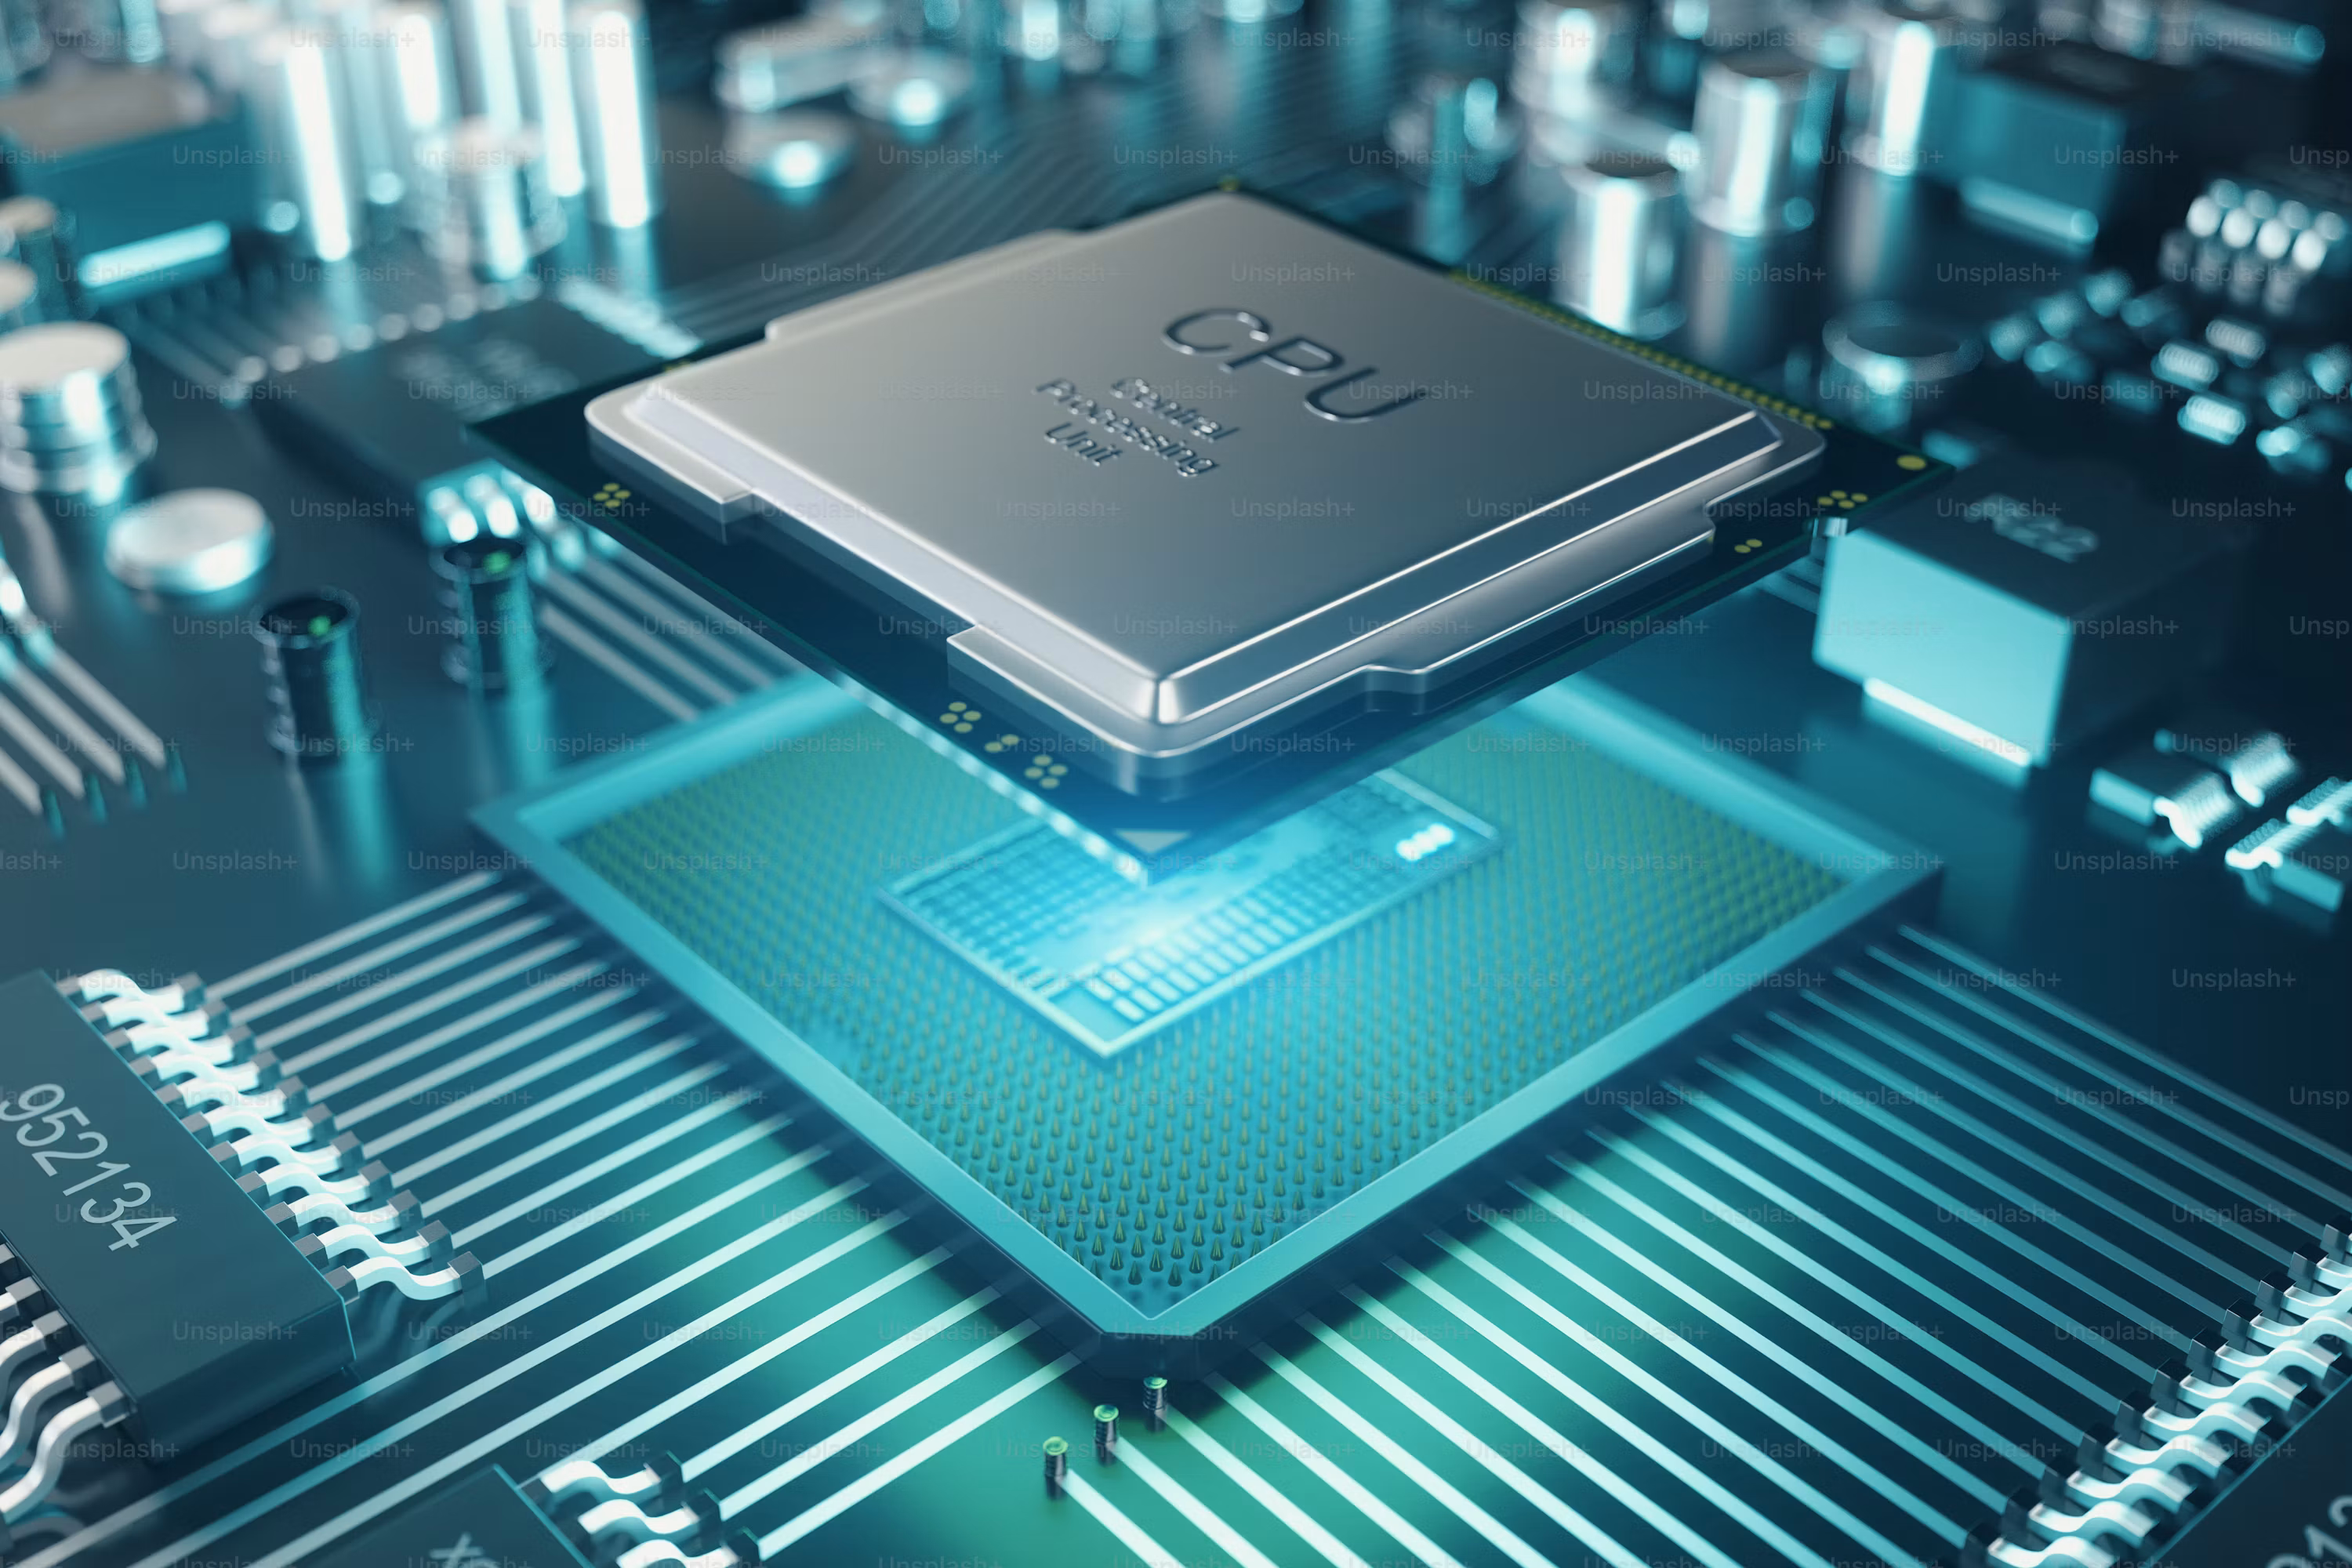
\includegraphics[height=1cm]{Images/top.png}} 
\fancyhead[R]{\thepage} 
\fancyhead[C]{\textit{\leftmark}} 

% Per avere l'intestazione anche nelle pagine iniziali dei capitoli
\fancypagestyle{plain}{
  \fancyhf{}
  \fancyhead[L]{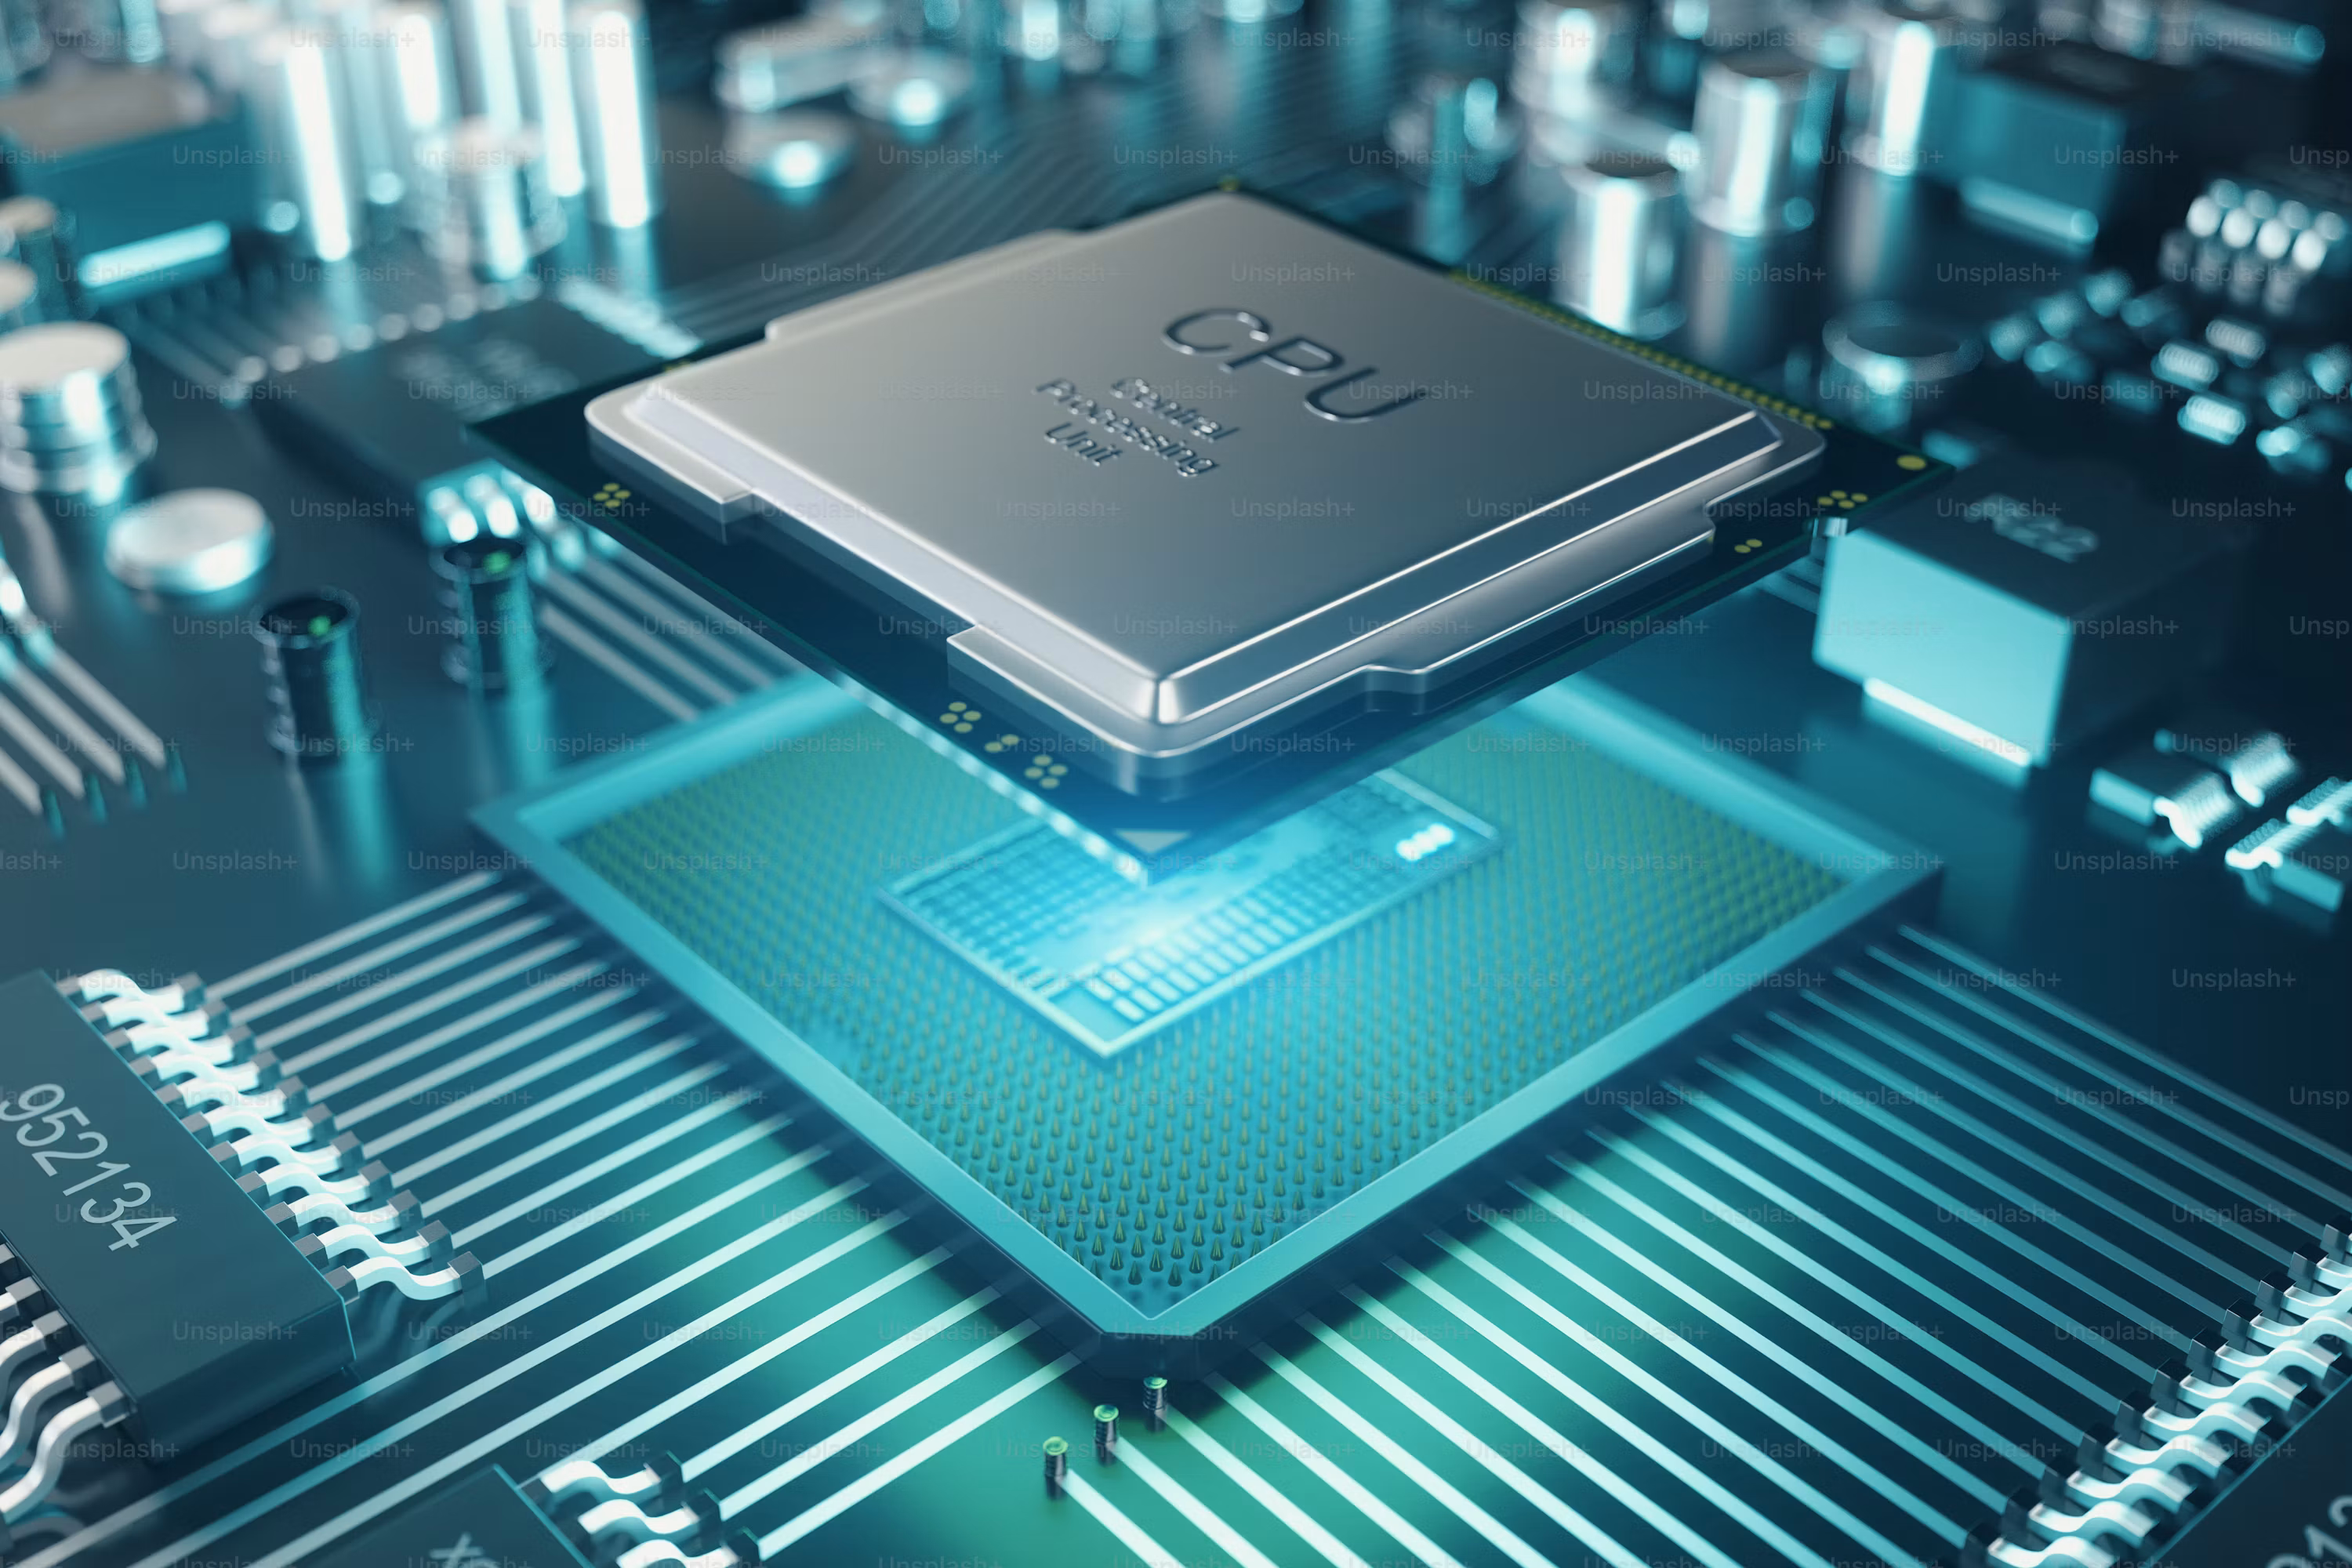
\includegraphics[height=1cm]{Images/top.png}}
  \fancyhead[R]{\thepage}
  \fancyhead[C]{\textit{\leftmark}}
  \renewcommand{\headrulewidth}{0.4pt}
}

% --- LINK CLICCABILI (Senza il backtick d'errore) ---
\usepackage[hidelinks]{hyperref} 
 

% --- COMANDI PERSONALIZZATI ---
\newcommand{\tikznode}[2]{%
  \ifmmode%
    \tikz[remember picture,baseline=(#1.base),inner sep=0pt] \node (#1) {$#2$};%
  \else
    \tikz[remember picture,baseline=(#1.base),inner sep=0pt] \node (#1) {#2};%
  \fi%
}
\tikzset{portnode/.style={circle, draw, inner sep=1pt, font=\scriptsize}}


\begin{document}
% --- PAGINA DEL TITOLO 
\begin{titlepage}
    \centering
    {\scshape\Large Università degli Studi "La Sapienza" \par} 
    \vspace{0.5cm}
    {\scshape\large Dipartimento di Ingegneria dell'Informazione, Elettronica e Telecomunicazioni \par}
    \vspace{0.5cm}
    {\scshape\large Corso di Laurea in Ingegneria Elettronica \par}
    \vspace{1.5cm}
    {\huge\bfseries Laboratorio Multidisciplinare\\ di Elettronica I\par}
    \vspace{0.35cm}
    {\Large\bfseries Relazione \NumeroRelazione\par}
    \vspace{0.35cm}
    {\Large\bfseries \TitoloRelazione\par}
    \vspace{1cm}
    {\large CFU:  6 \par} 
    \vspace{1.5cm}

    {\large Gruppo 18: \par}
    \vspace{0.2cm}
    {\Large Renato Bearzotti \par}
    {\Large Nicolò Falasca \par}
    {\Large Ionut Vlase }

    \vspace{0.4cm}
    \IfFileExists{Images/top.png}{%
        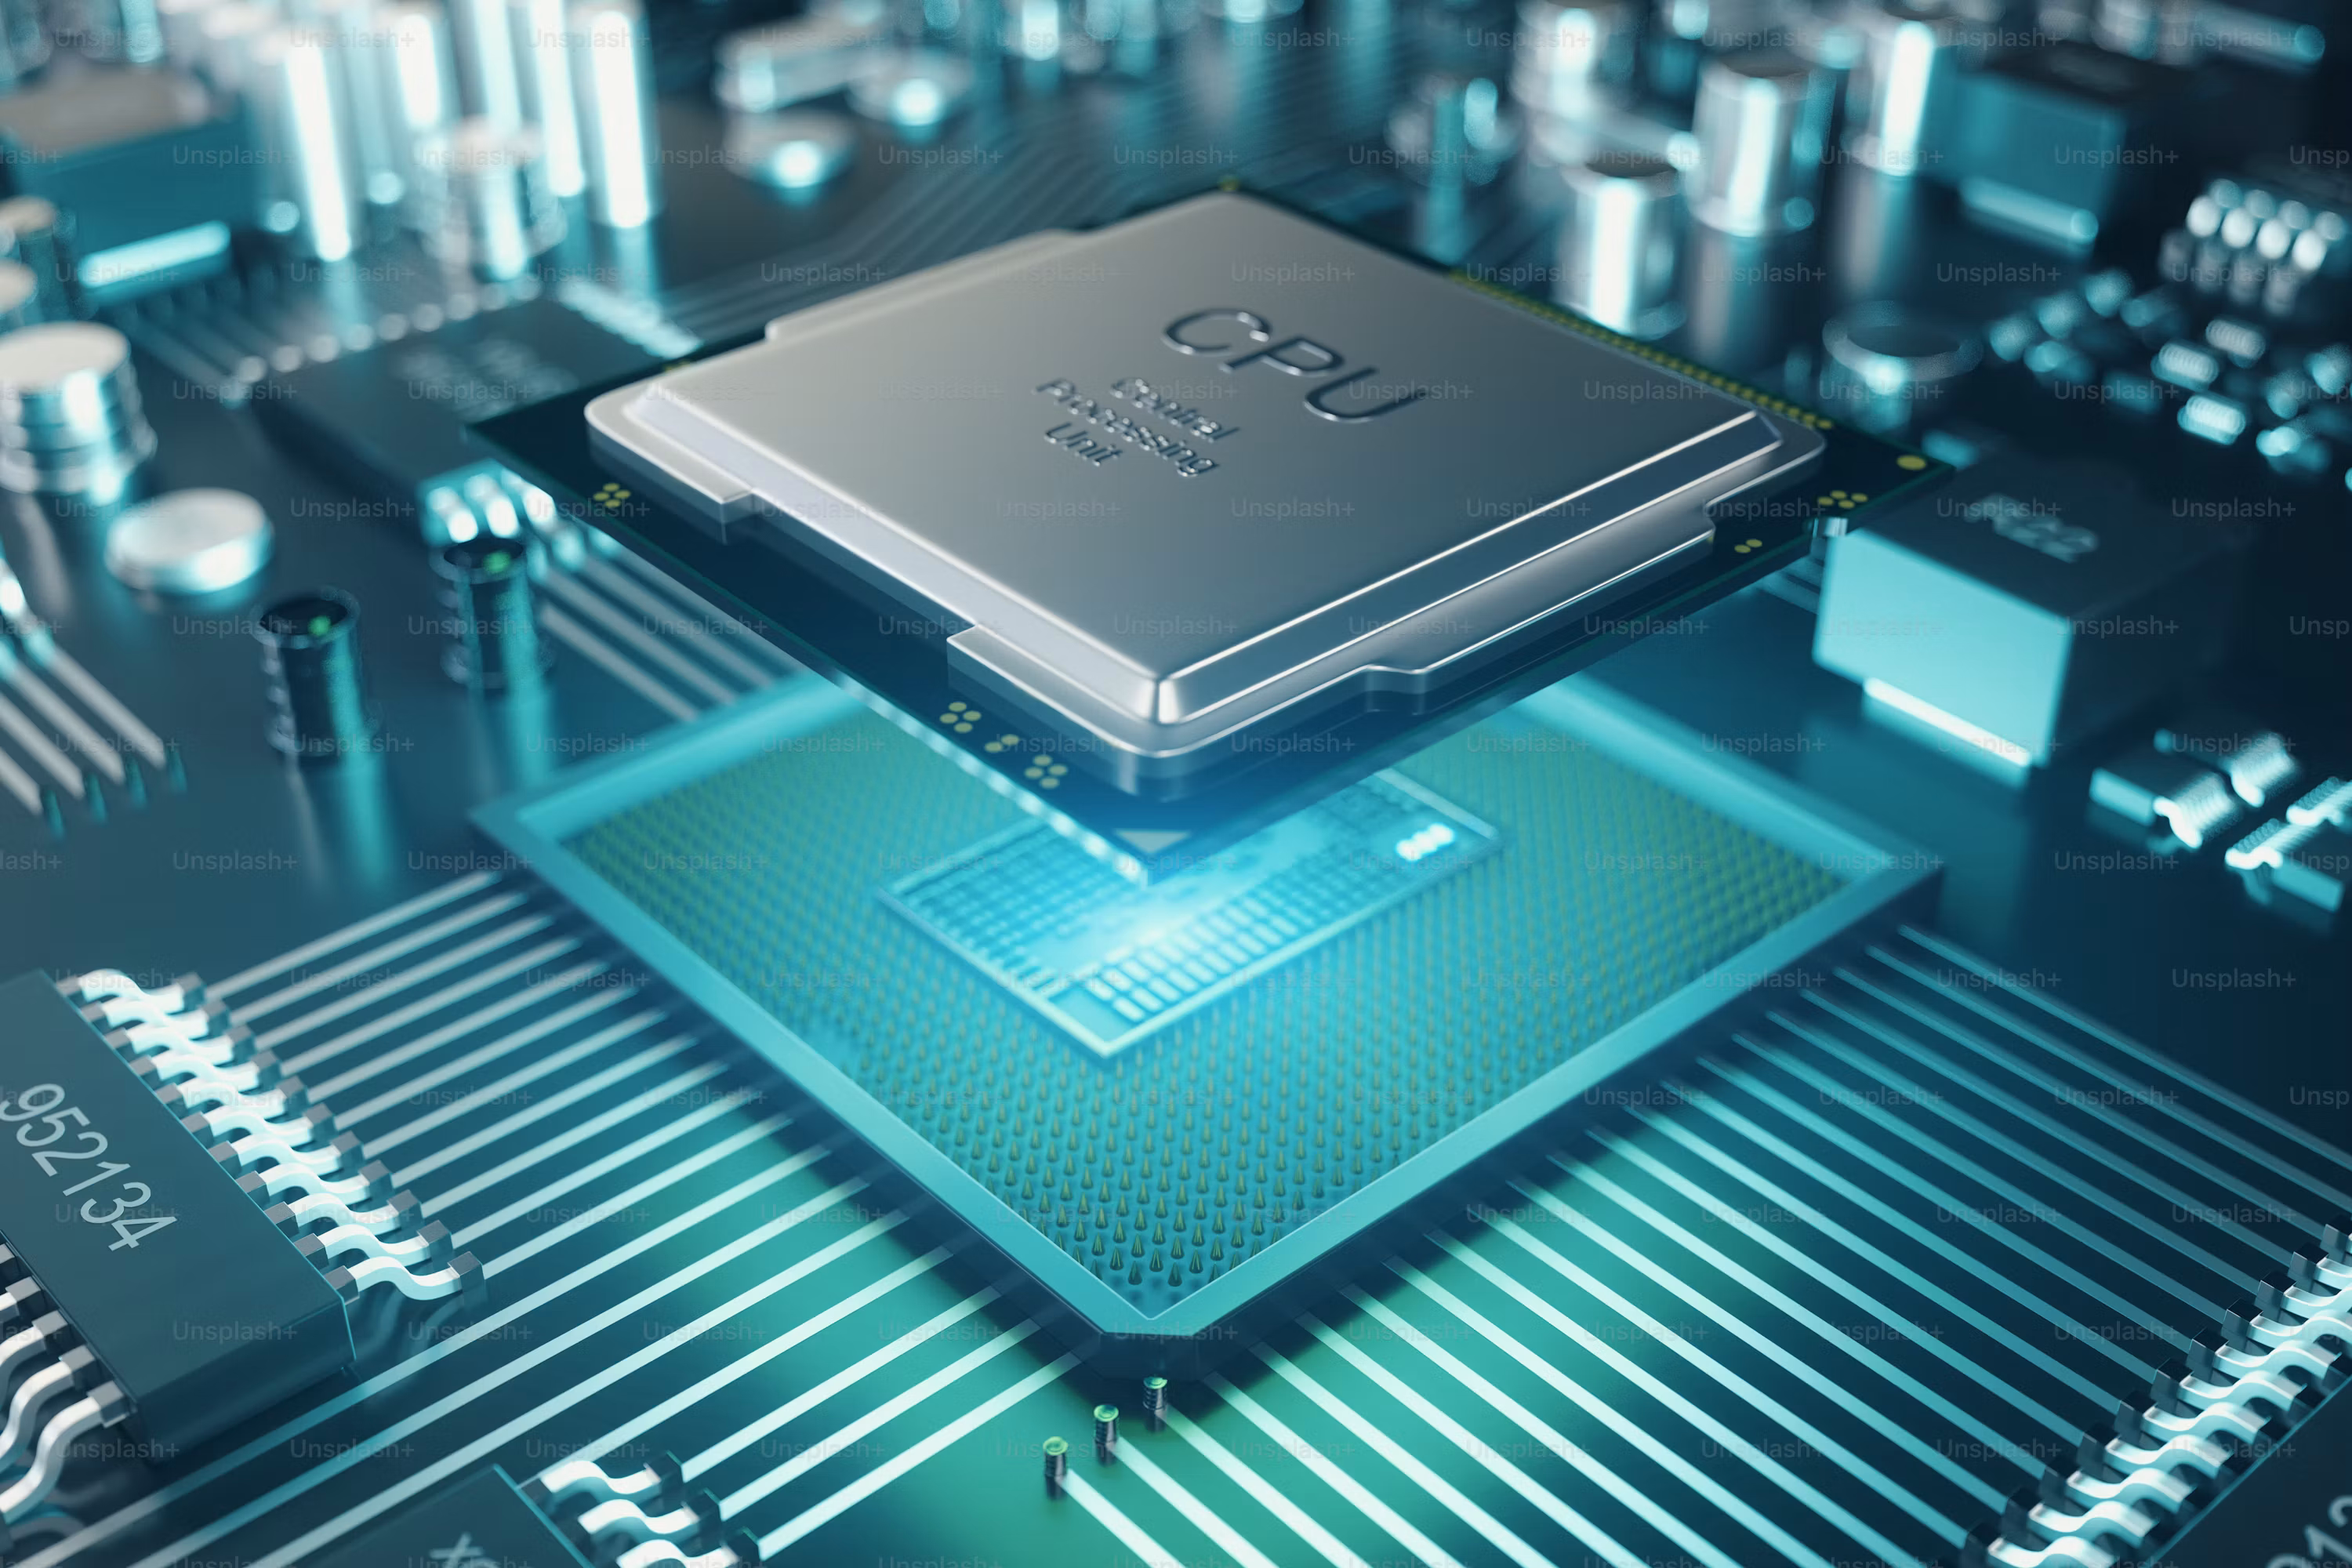
\includegraphics[width=3.5cm]{Images/top.png}\par
    }{}
    \vspace{0.25cm}
    \IfFileExists{Images/logo Sapienza (rgb).png}{%
        
\includegraphics[width=6.8cm]{Images/logo Sapienza (rgb).png}\par
    }{}
    \vspace{0.6cm}

    % Professori allineati a destra
    \begin{minipage}[t]{\textwidth}
        \begin{flushright}
            \large
            \textbf{Professori:}\\
            Andrea Mostacci\\
            Stefano Pisa\\
            Pasquale Tommasino
        \end{flushright}
    \end{minipage}

    \vfill
    {\large Anno Accademico 2026-2027 \par}
\end{titlepage}


\frontmatter 
\tableofcontents

\mainmatter
 


\chapter{Filtro passa banda}
 
\section{Misura del modulo di del paramtro di trasmissione in banda senza calibrazione}
Siamo partiti misurando il modulo del parametro di trasmissione, $|S_{21}|$ intorno alla banda del filtro, tra 4.92 e 5.35 GHz.
\begin{figure} [H]
    \centering
    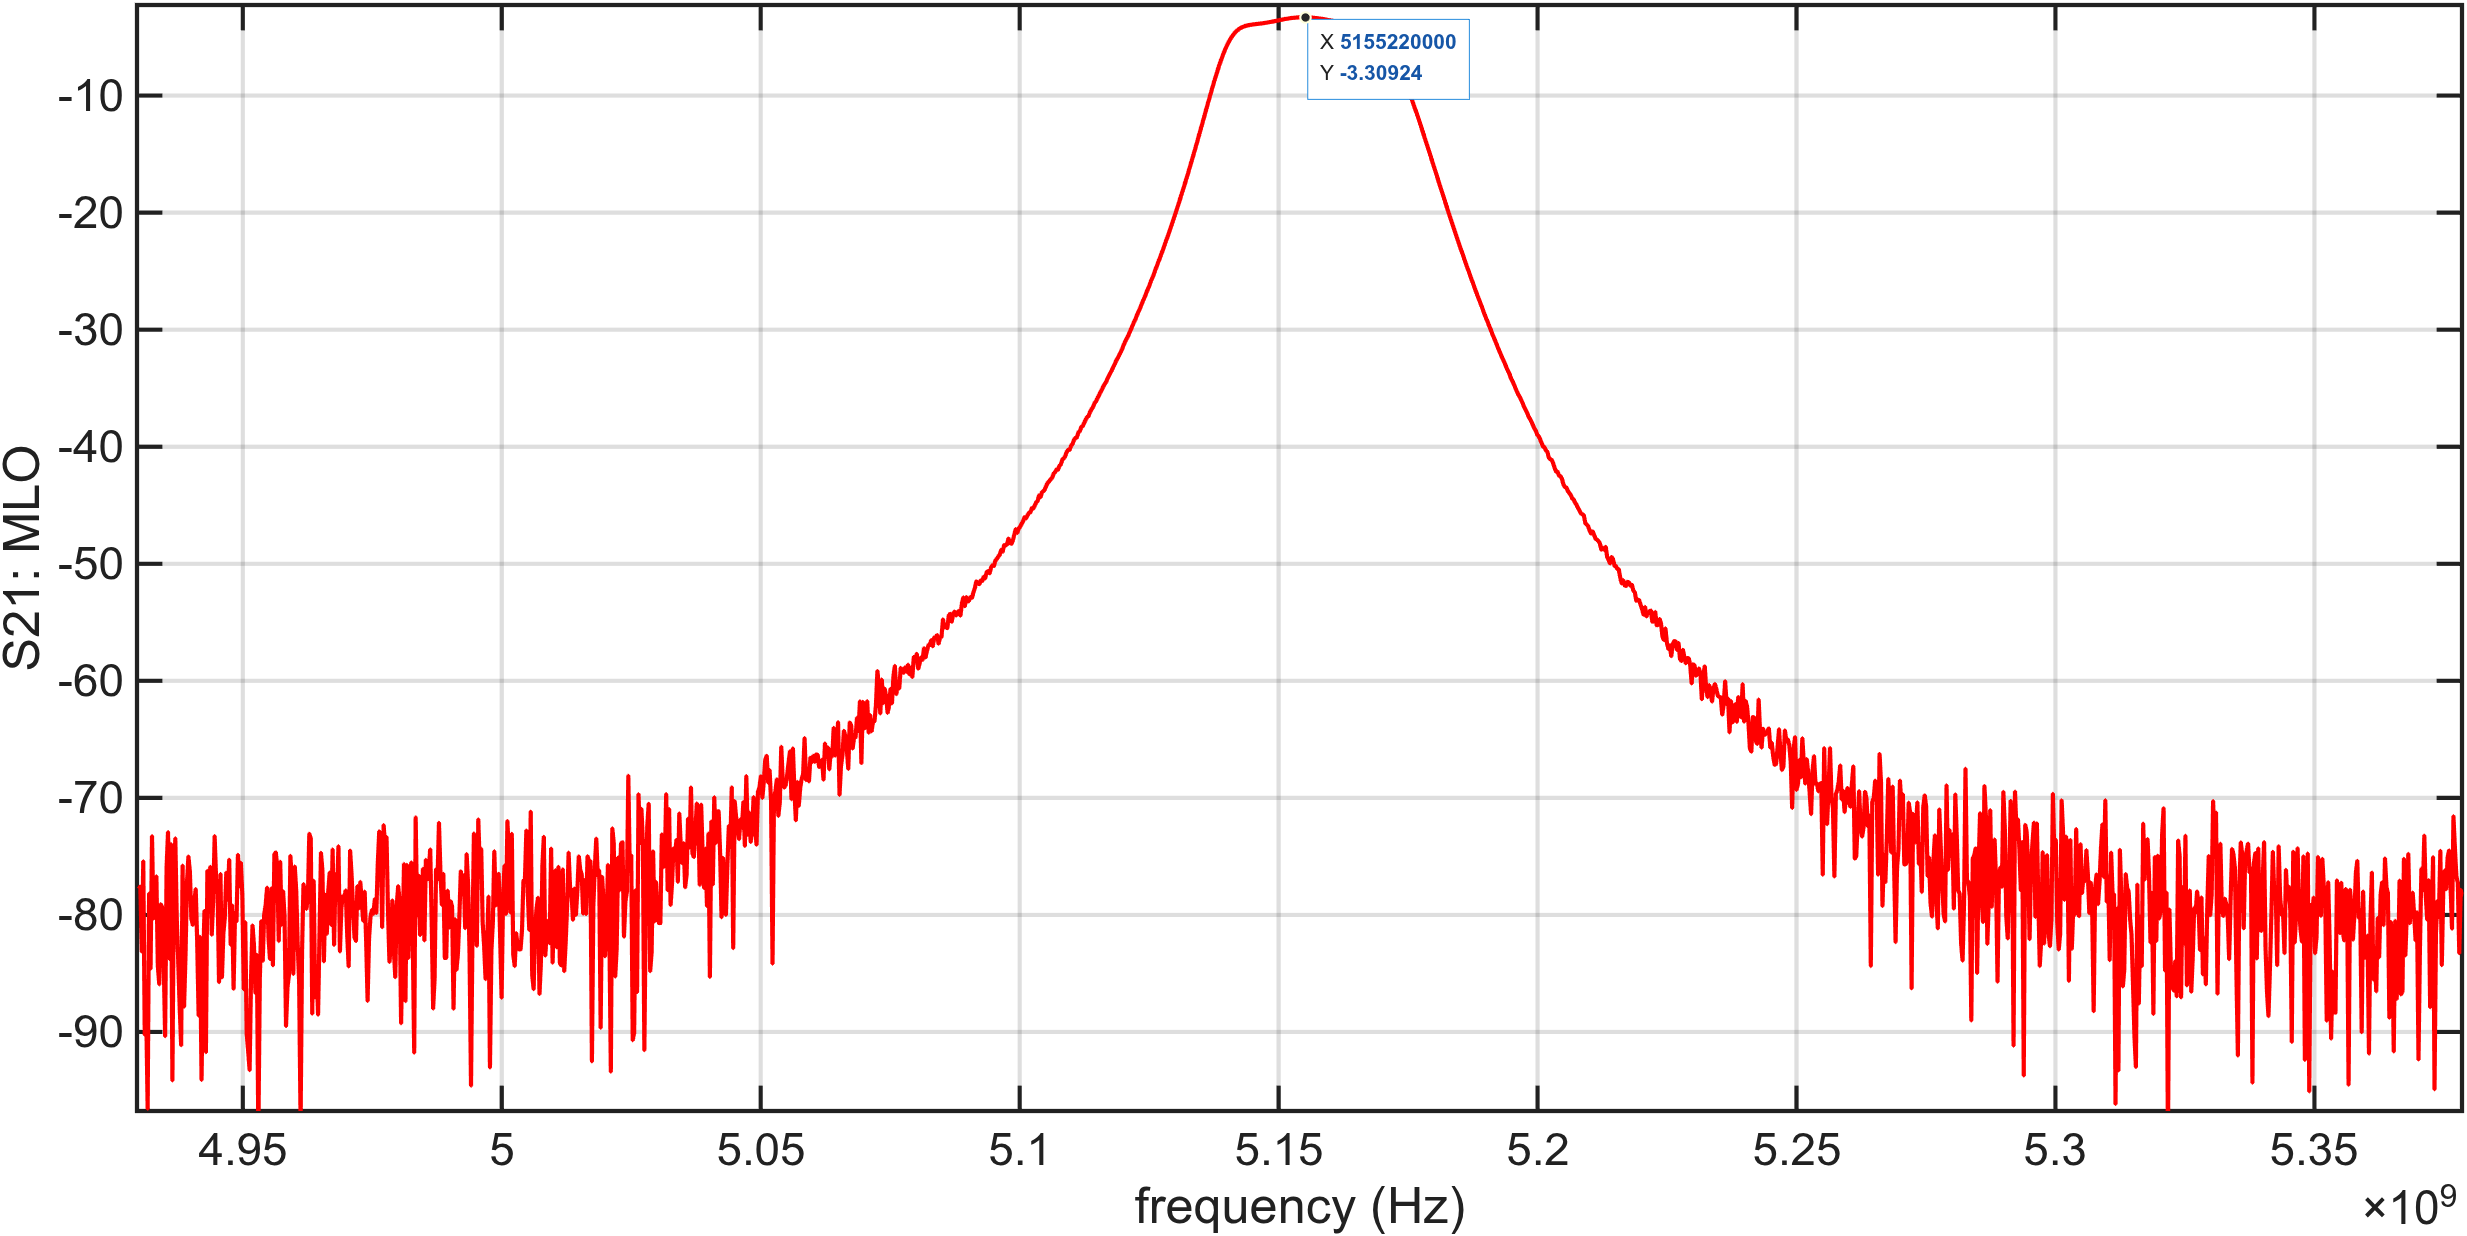
\includegraphics[width=0.6\textwidth]{./Images/Relazione7_Foto/1_1_Misura_S21_filtro_senza_calir.png}
    \caption{Misura del modulo di del paramtro di trasmissione in banda senza calibrazione.}
\end{figure}
Come ci aspettiamo, abbiamo un picco a -3dB nella regione dove passa il segnale e una discesa molto ripida fouri dalla banda. abbiamo deciso di mostrare uno span ampio rispetto alla banda del filtro, per mostare il suo intero adamento fino a che non rimane solo rumore. 

\section{Misura del modulo di del paramtro di trasmissione in banda con calibrazione e confronto tra misura con e senza calibrazione}
Abbiamo attivato la calibrazione, valida tra 10MHz e 9 GHz e abbiamo misurato nuovamente modulo di del paramtro di trasmissione, in modo da valutare la differenza introdotta dalla calibrazione nella misura.

\begin{figure} [H]
    \centering
    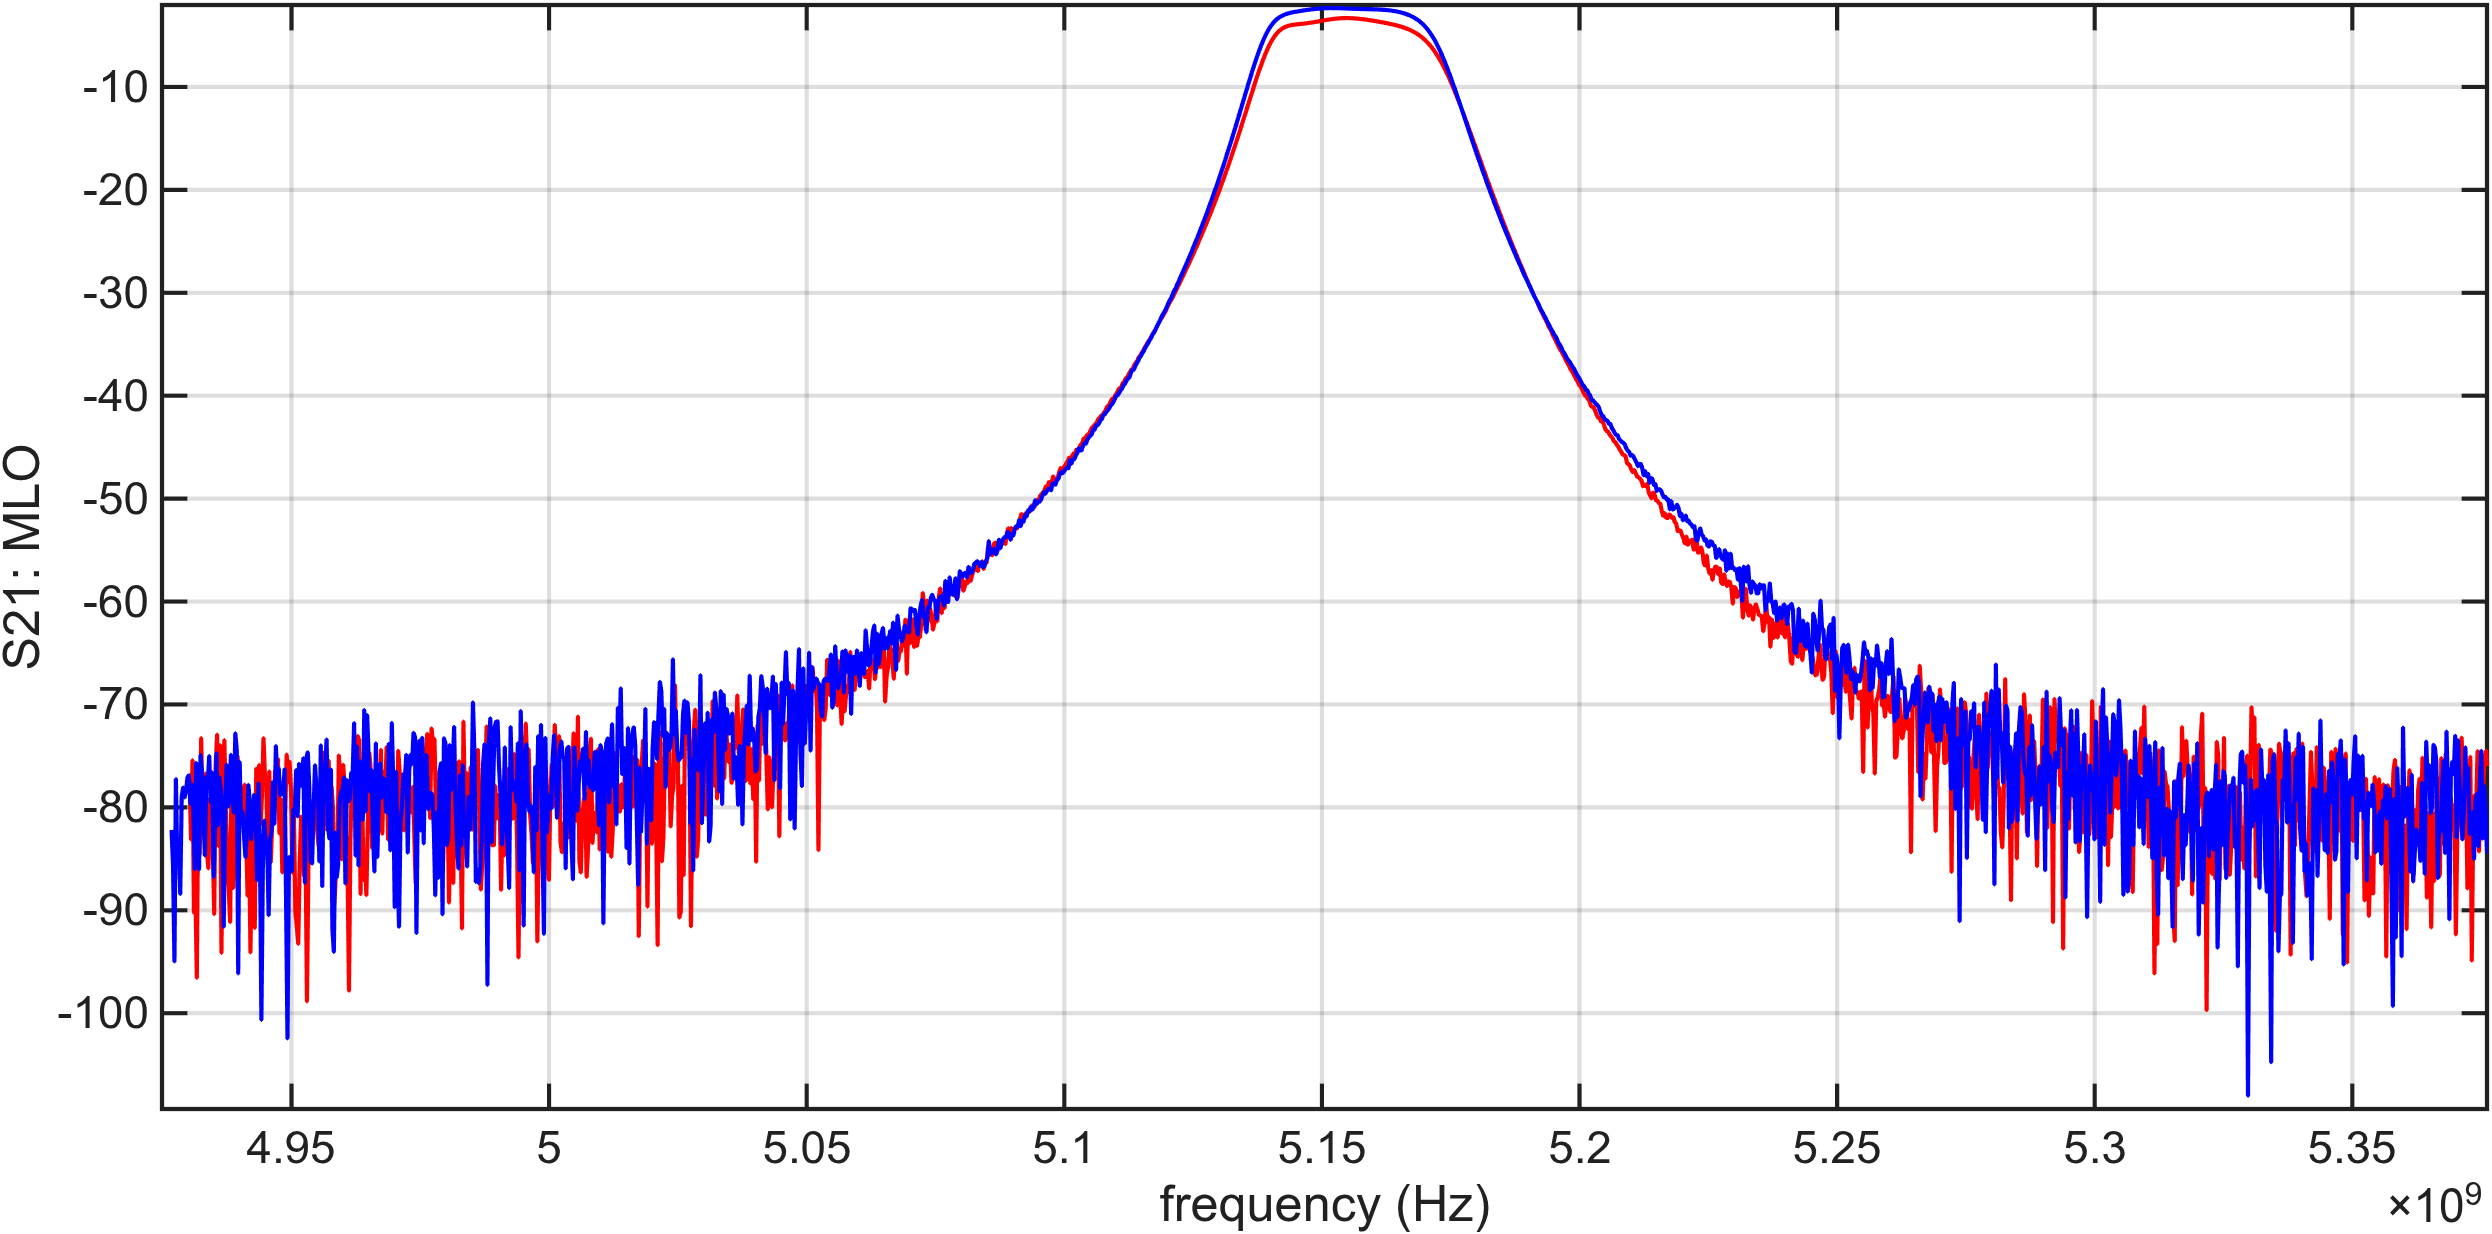
\includegraphics[width=0.6\textwidth]{./Images/Relazione7_Foto/1_2_Misura_S21_filtro_con_calir.png}
    \caption{Misura del modulo di del paramtro di trasmissione in banda con calibrazione attiva (blu) e senza calibrazione (rosso).}
\end{figure}
Come è facile notare, le due misure sono molto vicine tra loro, e si sovrappongono quasi completamente. L'unica differenza che a reputiamo importante sottolineare è il valore di picco, ossia il valore in banda, che sale da circa -3.3dB a -2.4dB, quindi abbiamo circa 1dB in più con calibrazione attiva, legato 
alle perdite del cavo, che vengono valutate con la calibrazione attiva.


\section{Valutazione della banda -3dB e -60dB}
Dalla misurazione di $|S_{21}|$ con calibrazione attiva abbiamo valutato la banda -3dB e -60dB tramite lo strumento che ci permette di misurare tutto senza post elaborazione.
\\I risultati sono i seguenti:
\begin{center}
\begin{tabular}{ |c|c|c| }
    \hline
    Banda -3dB (MHz) & Banda -60dB & Q \\ \hline
    33.019 & 163.61 & 156.13 \\
    \hline
\end{tabular}
\end{center}
Essendo la risposta in frequenza centrata a 5.17GHz, possiamo concludere che il filtro è progettato per lavorare tra circa 5.14 e 5.20 GHz, con riferimento alla banda -3dB.
\\In tabella abbiamo valutato il fattore di qualità rispetto alla banda -3dB, per mantenere la definizione standard di fattore di qualità Q.
\\Ovviamente il valore di Q è molto inferiore rispetto a quello dei risonatori, che sono elementi progettati per avere il massimo di Q. 

\section{Misura dei parametri della matrice di scattering}
Siamo passati poi a valutare gli altri coefficienti della matrice di scatterig, inserendoli in 2 grafici, uno per i parametri di riflessione e uno per i parametri di trasmissione. 
\\Per i parametri di riflessione:
\begin{figure} [H]
    \centering
    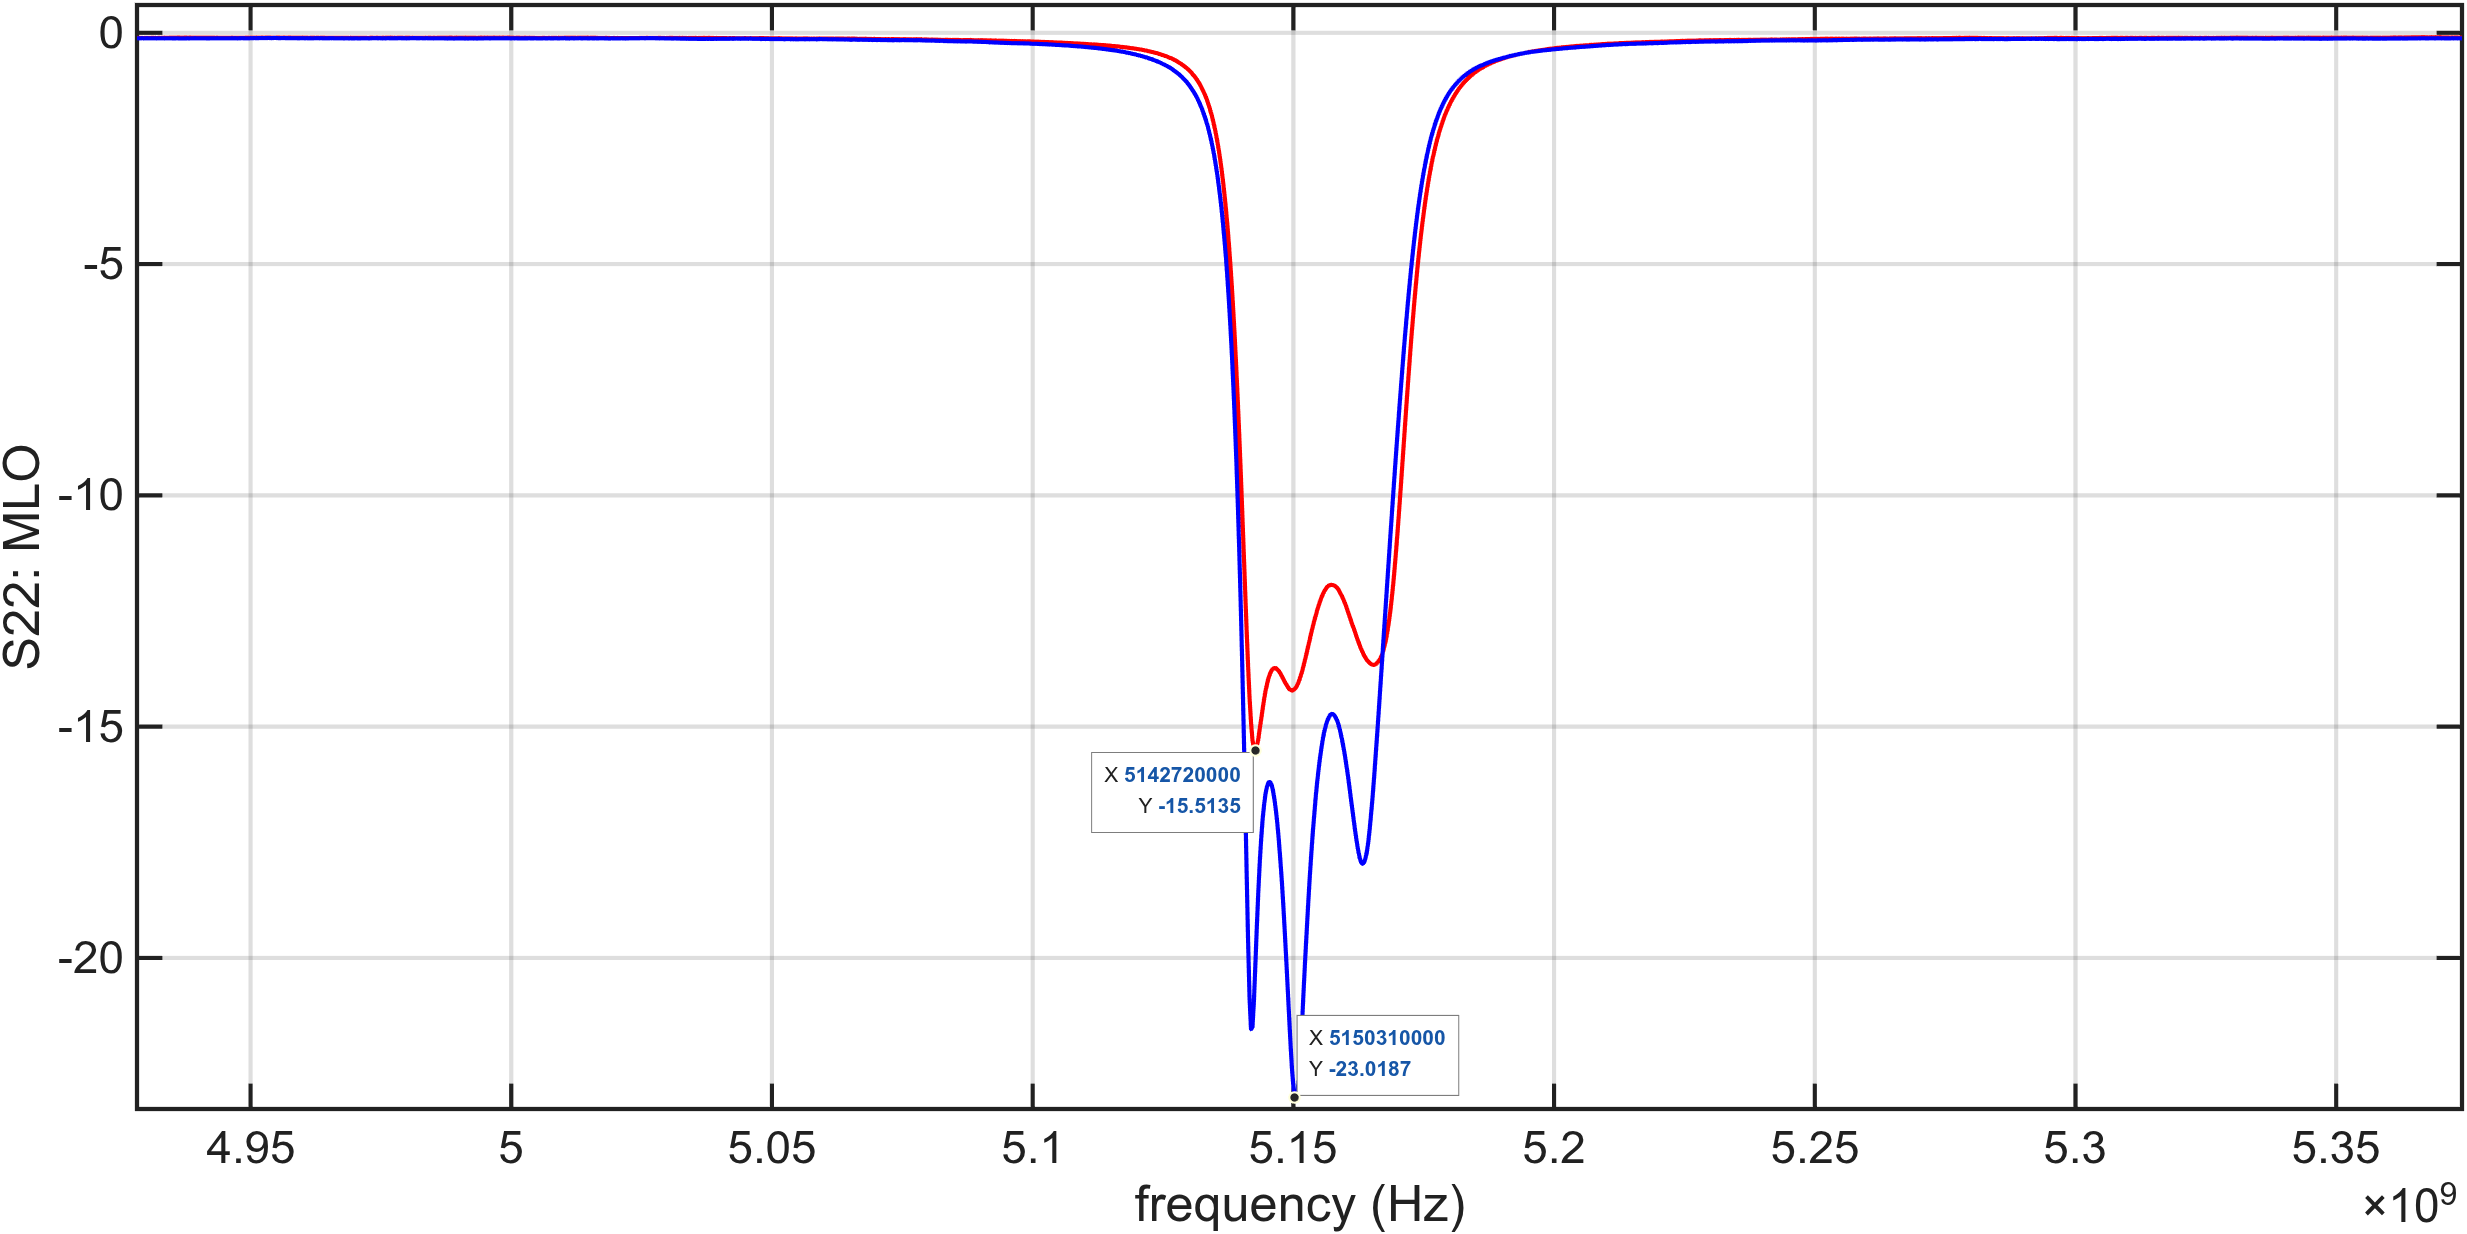
\includegraphics[width=0.6\textwidth]{./Images/Relazione7_Foto/1_4_S11_e_S22.png}
    \caption{Misura del modulo di $S_{11}$ (rosso) e del modulo di $S_{22}$ in blu.}
\end{figure}
Dalla misura di nota che il coefficiente di riflessione alla porta 2 è molto inferiore, circa 10dB in meno di valore minimo.
\\I due coefficienti in banda assumono comunque valori molto piccoli, come ci aspettavamo da un filtro, che deve far passare tutto il segnale nella banda prestabilita.
\\Per i coefficienti di trasmissione invece:
\begin{figure} [H]
    \centering
    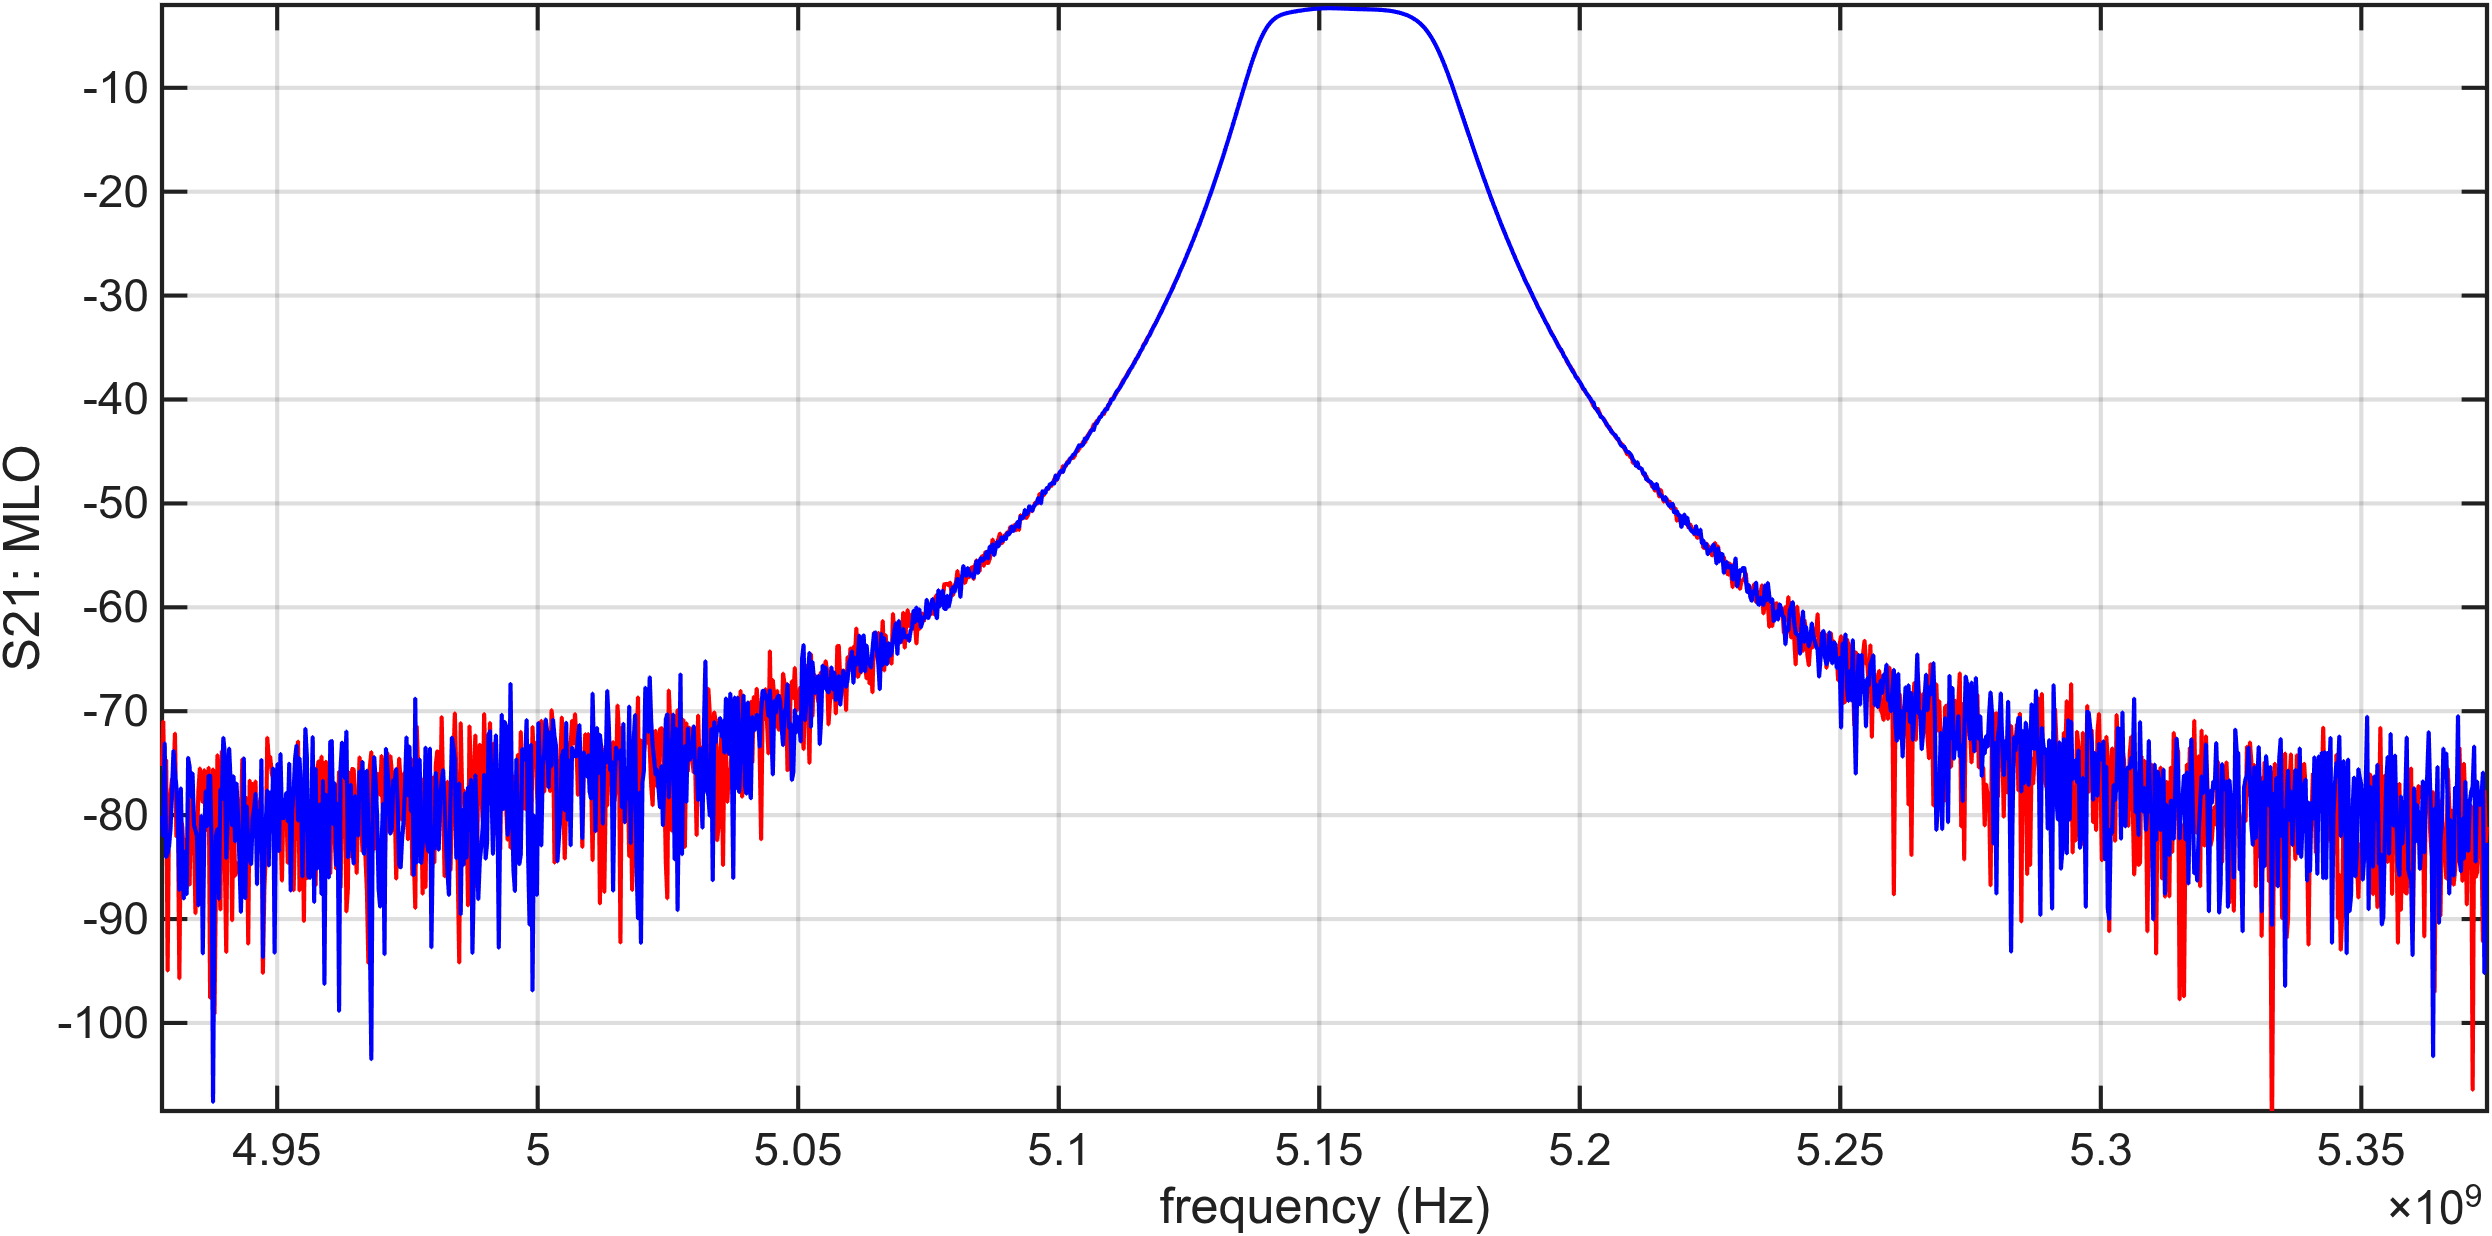
\includegraphics[width=0.6\textwidth]{./Images/Relazione7_Foto/1_4_S12_e_S21.png}
    \caption{Misura del modulo di $S_{12}$ (rosso) e del modulo di $S_{21}$ in blu.}
\end{figure}
Anche in questo caso troviamo un risultato atteso, i due grafici in banda si sovrappongono perfettamente in banda, cosa ovvia per un componente reciproco come un filtro passa-banda.
\\L'andamento, come visto anche nel primo paragrafo, è quello di un filtro passa-banda, che fa passare il segnale sono in banda, e la cui risposta in frequenza decresce molto rapidamente fuori banda.

\section{Misura della fase del parametro di trasmissione e del ritardo introdotto dal filtro}
Abbiamo misurato la fase di $S_{21}$ in formato wrapped. Abbiamo poi fatto l'unwrap ed eseguito il linear fit per ricavare la pendenza.
\\Il risultato è il seguente:
\begin{figure} [H]
    \centering
    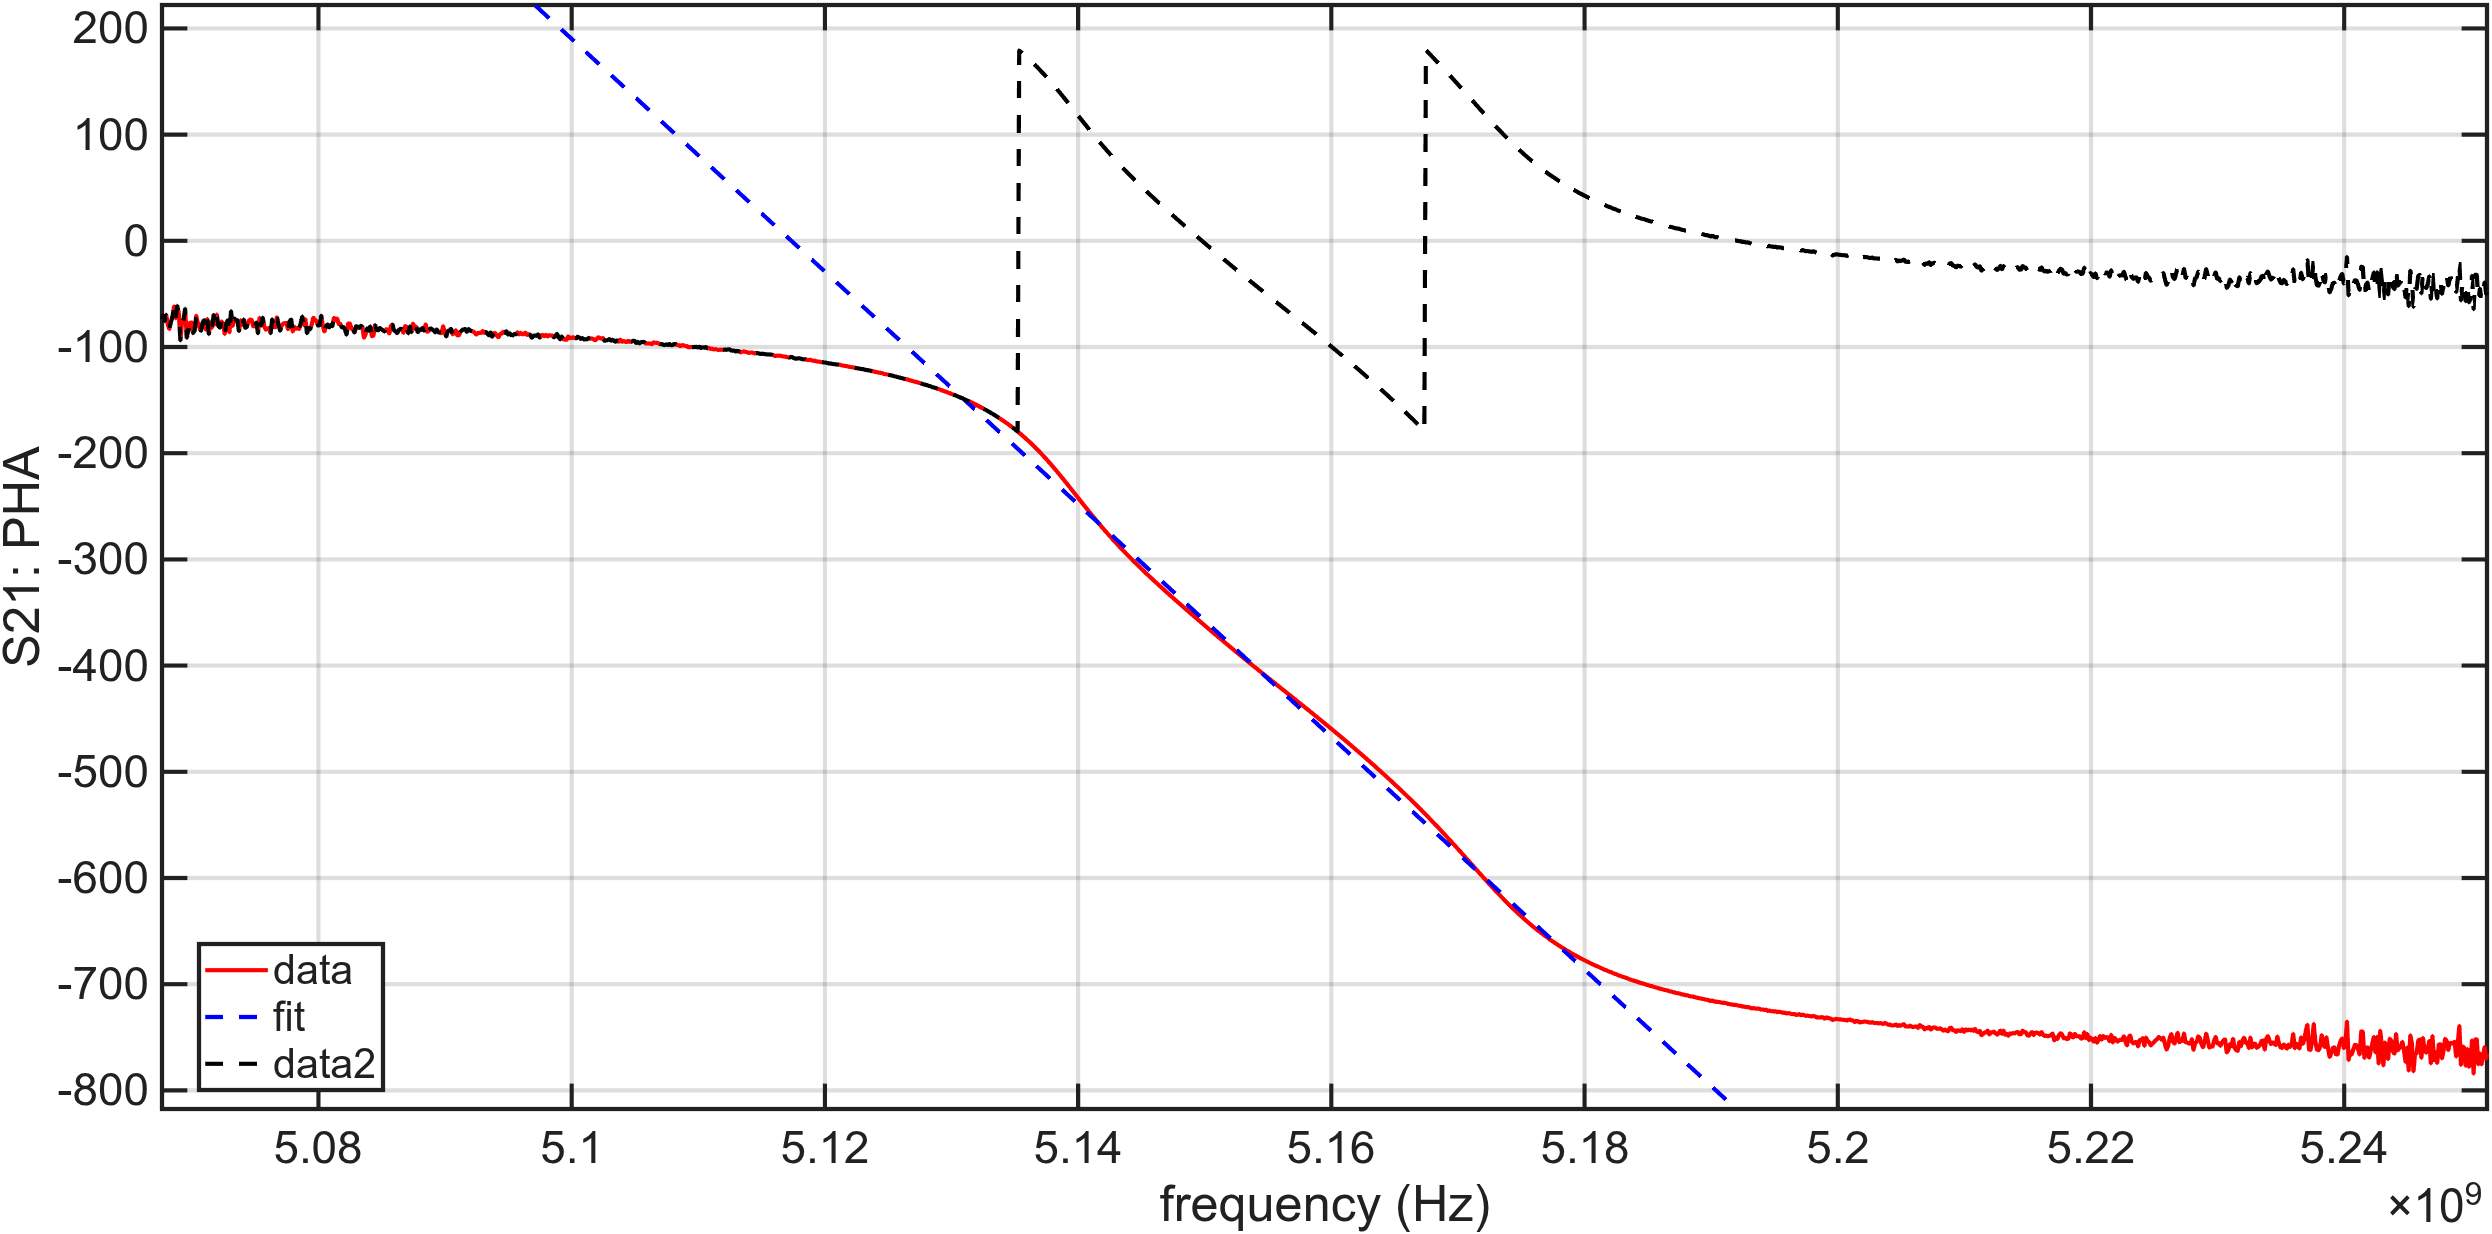
\includegraphics[width=0.6\textwidth]{./Images/Relazione7_Foto/1_5_fase_S21.png}
    \caption{Misura della fase in formato wrapped (nero), unwrapped (rosso) e linear fit della fase (blu).}
\end{figure}
Dal linear fit otteniamo:
\begin{equation}
    \overline{p}=-1.095546420678454\cdot 10^{-05} \quad °/Hz
\end{equation}
\begin{equation}
    \sigma_p= 1.065250129543955\cdot 10^{-7} \quad °/Hz
\end{equation}
Da queste troviamo il ritardo $\tau$:
\begin{equation}
    \overline{\tau}=\frac{-\overline{p}}{360°}=-3.0432\cdot 10^{-8} \quad s
\end{equation}
\begin{equation}
    \sigma_{\tau}= \frac{\sigma_p}{360°}   =2.9590\cdot 10^{-10} \quad s
\end{equation}
E quindi possiamo concludere:
\begin{equation}
    \tau=3.043 \pm 0.030   \cdot 10^{-8} \quad s
\end{equation}
Abbiamo poi misurato il ritardo anche dallo strumento. Il risultato è il seguente.
\begin{figure} [H]
    \centering
    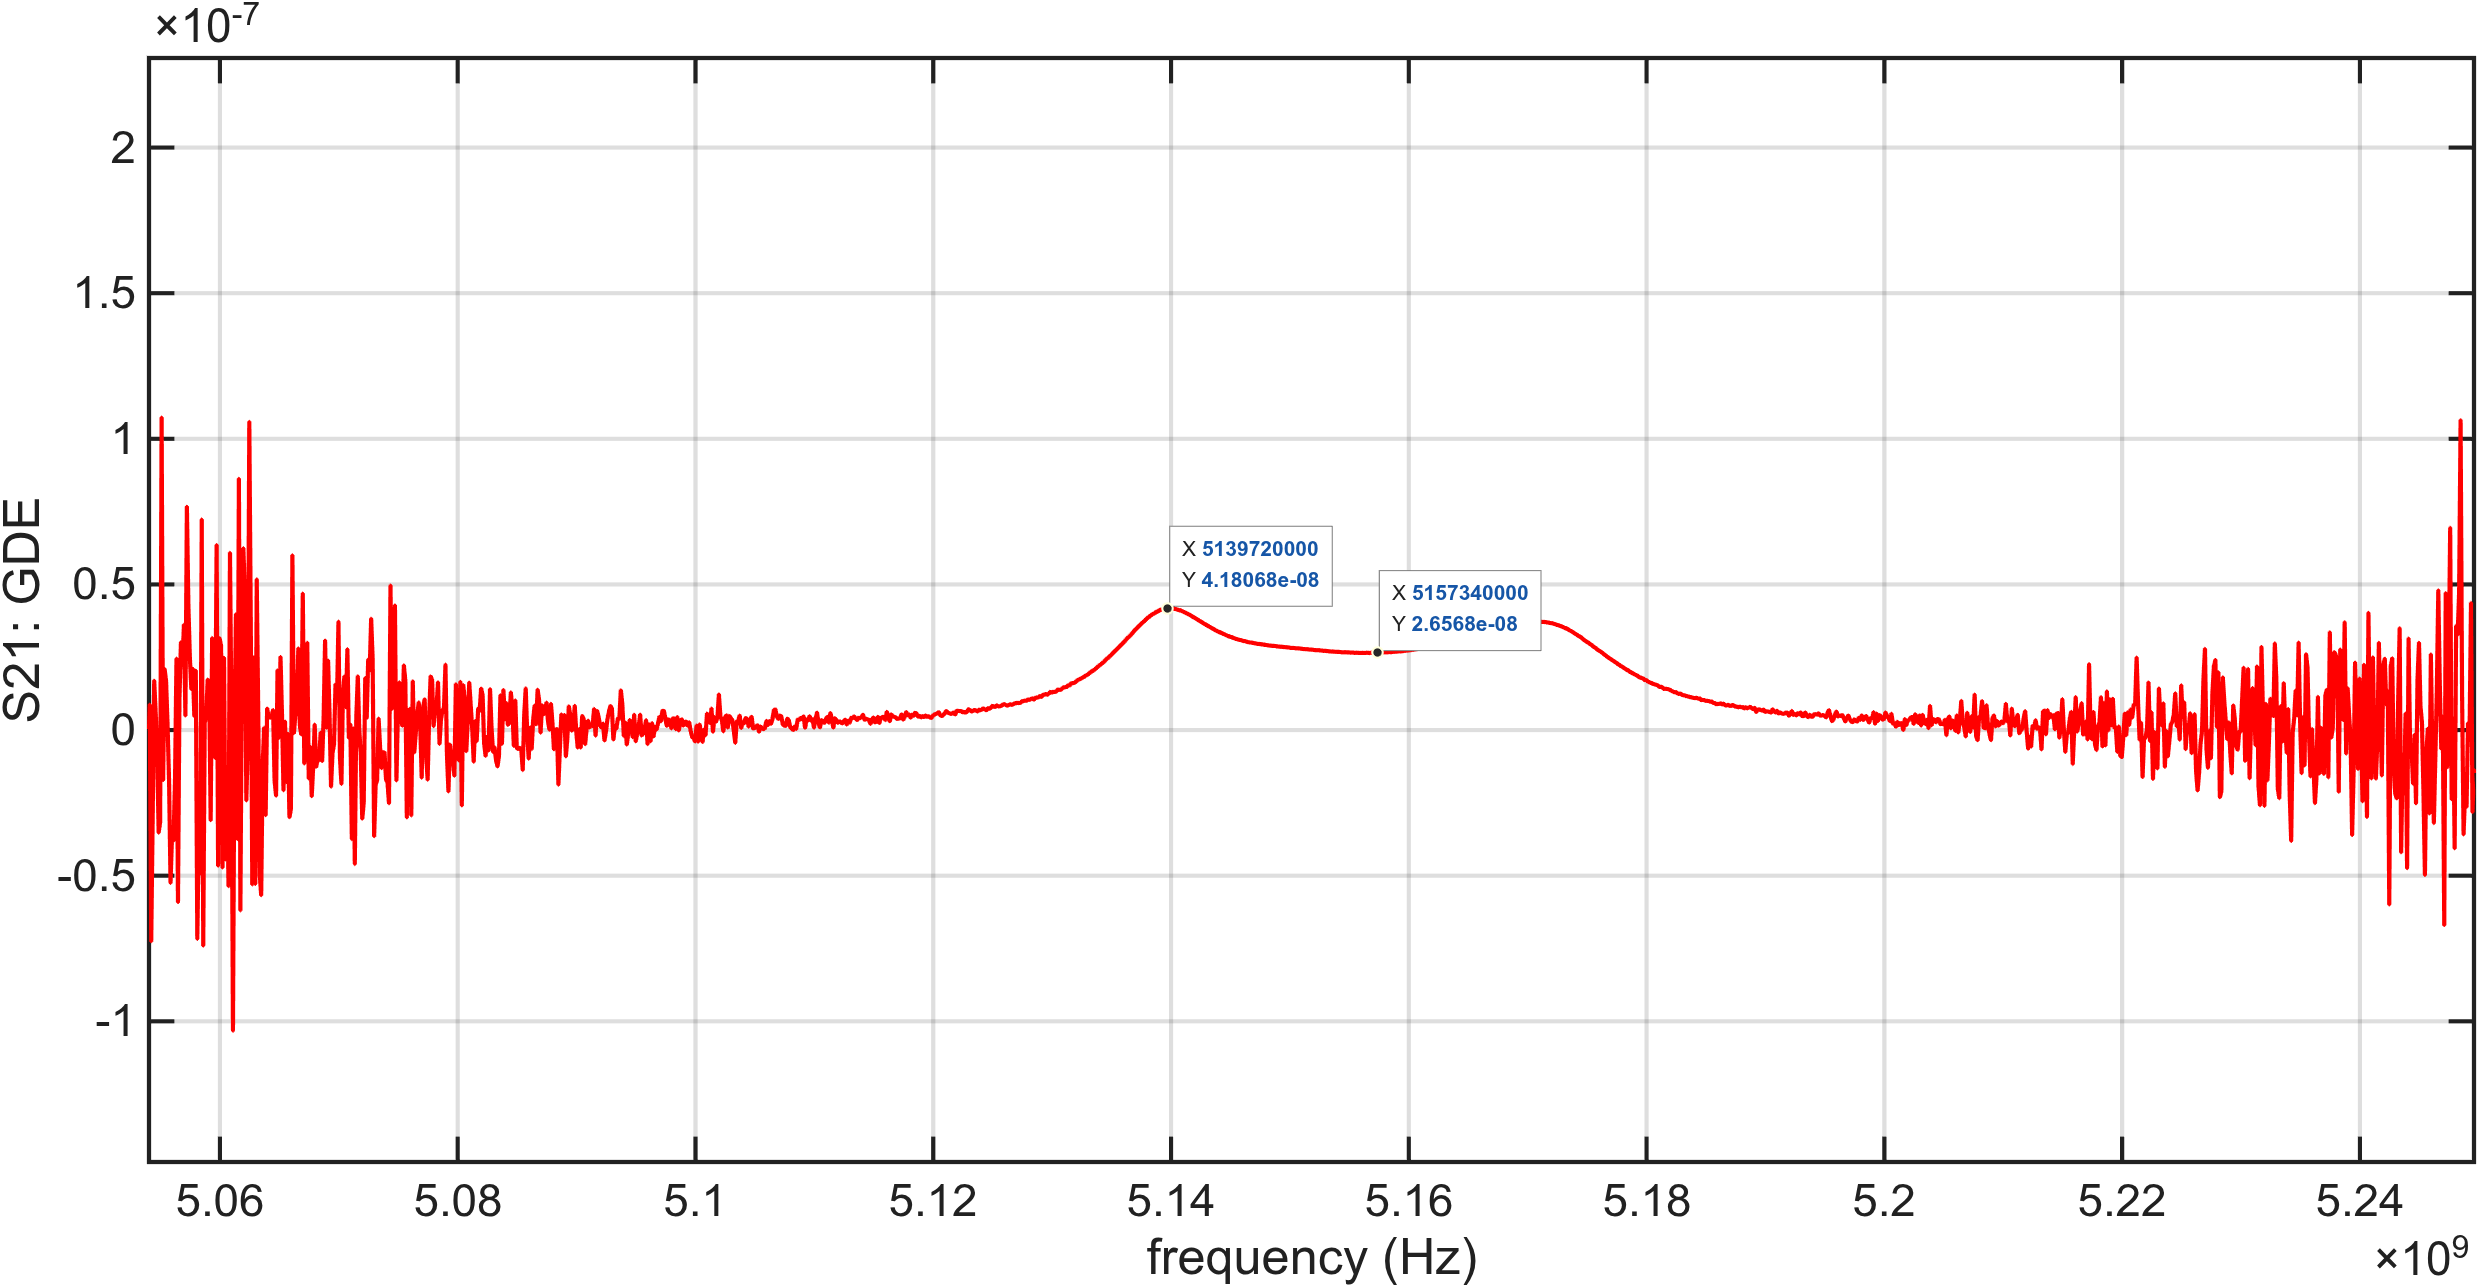
\includegraphics[width=0.6\textwidth]{./Images/Relazione7_Foto/1_5_misura_delay.png}
    \caption{Misura del ritardo introdotto dal filtro.}
\end{figure} 
In figura abbiamo evidenziato il valore massimo (41.81 ns) e minimo (26.57 ns) del ritardo in banda. 
\\Il valore trovato tramite linear fit si trova tra questi due valori ottenuti dallo strumento. Possiamo quindi ritenere il valore ottenuto tramite linear fit valido e coerente, poiché è un valore trovato come valor medio in
banda.


\chapter{Giunzione a T, divisore di potenza}

\section{Giunzione a T: matrice di scattering misurata e teorica}
Abbiamo misurato con lo struemnto tutti i parametri della matrice di scatterig. Ricordiamo che per reciprocità dello strumento $S_{21}=S_{12}$, $S_{31}=S_{13}$ e $S_{23}=S_{32}$, quindi bastano 6 misure per ottenere la matrice. Ovviamente tutte le misure sono state prese con l'altra porta chiusa su un carico adatatto.
\[
\begin{pmatrix}
-9.58 \cdot e^{107.69} & -3.55 \cdot e^{-63.84} & -3.66 \cdot e^{-64.28} \\
-3.55 \cdot e^{-63.84} & -9.51\cdot e^{112.17} & -3.62\cdot e^{-63.04} \\
-3.66 \cdot e^{-64.28} & -3.62 \cdot e^{-63.04} & -9.81 \cdot e^{113.14}
\end{pmatrix}
\]
Come ci aspettavamo, la matrice ha coefficiente di riflessione in ingresso alle tre porte molto piccolo (meno di -9dB per ogni porta), e i coefficienti di trasmissione pari a circa -3dB, quindi 
la potenza che entra in ogni porta viene ripartita equamente alle altre due porte (-3dB equivale a dividere per due in lineare).

\section{Divisiore di potenza: matrice di scattering misurata e teorica}
Anche in questa misurazione valgono le considerazioni del paragrafo precedente, quindi la reciprocità della marice, e l'aveer adattato la sempre una porta per prendere le misure.
\[
\begin{pmatrix}
 -31.23 \cdot e^{-59.05} & -6.06 \cdot e^{-105.43} & -6.21 \cdot e^{-112.77} \\
-6.06 \cdot e^{-105.43} & -35.16\cdot e^{-10.01} & -6.19\cdot e^{-111.45} \\
-6.21 \cdot e^{-112.77} & -6.19\cdot e^{-111.45} & -23.22 \cdot e^{-25.06}
\end{pmatrix}
\]

\chapter{Circolatore}

\section{Valutazione della banda -3dB}

\section{Matrice di scattering}

\section{Misura del ritardo}




\chapter{Accoppiatore direzionale}

\section{Insertion loss}

\section{Isolamento}

\section{Accoppiamento}

\section{Direttività}

\section{Return Loss}




\chapter{Accoppiatore ibrido}

\section{Accoppiamento tra la porta 1 e le porte 3 e 4}

\section{Isolamento tra la porta 1 e la porta 2}

\section{Misura della fase tra la porta 1 e le porte 3 e 4, con ricerca del tipo di accoppiatore (90° o 180°)}



\chapter{Amplificatore e sweep di potenza}

\section{Misura del guadagno e del return loss di inpu e output}

\section{Valutazione della banda -3dB del guadagno e della banda -10dB del return loss}
\subsection{Banda -3dB del guadagno}

\subsection{Banda -10dB del return loss}

\section{Misura del modulo del parametro di trasmissione con sweep di potenza e valutazione del punto di compressione a 1dB}

\section{Misura del coefficiente di riflessione d'ingresso e della ressiitenza in funzione della potenza}

\end{document}
